\documentclass[12pt]{article}
\usepackage[utf8]{inputenc}
\usepackage[spanish]{babel}
\usepackage[margin = 1.5cm]{geometry}
\usepackage{mathtools}
\usepackage{graphicx}
\usepackage{anysize}
\usepackage{multicol}
\usepackage{amsmath}
\usepackage{amssymb}
\usepackage{enumerate}
\usepackage{stackrel}
\usepackage{mathrsfs}
\usepackage{parskip}


    \title{Fundamentos de Bases de Datos \\Tarea 1:     Conceptos básicos}

    \author{Teresa Becerril Torres 315045132\\
        Miguel Torres 315300442\\
        Nicole Romina Traschikoff García 315164482\\
        \\}
    \date{23 de Agosto del 2019}

    \begin{document}
        \maketitle

    \section{Conceptos generales.}
          \begin{enumerate}[a. ]
            \item ¿Por qué elegirías almacenar datos en un \textbf{sistema de base de datos} en lugar de simplemente almacenarlos
            utilizando el \textbf{sistema de archivos} de un sistema operativo? ¿En qué casos no tendría sentido utilizar un sistema
            de base de datos?
            \item ¿Qué \textbf{ventajas} y \textbf{desventajas} encuentras al trabajar con una \textbf{base de datos}?
            \item Investiga cuáles serían los distintos tipos de usuarios finales de una base de datos, indica las principales
            actividades que realizaría cada uno de ellos.
            \item Explica las diferencias entre la \textbf{independencia de datos física} y \textbf{lógica}. ¿Cuál es más difícil de lograr y
            por qué?
            \item ¿Qué es un \textbf{diccionario de datos} y por qué es importante para el SMBD?
            \item Indica las principales características de los modelos de datos más representativos. ¿Cuáles serían las
            diferencias entre los modelos relacional, orientado a objetos, semiestructurado y objeto-relacional?
            \item Elabora una \textbf{línea de tiempo}, en dónde indiques \textbf{los principales hitos} en el desarrollo de las BDs.


                  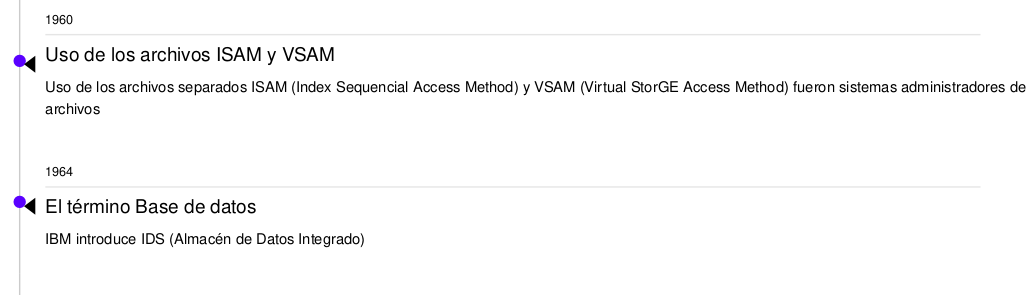
\includegraphics[width=\textwidth]{imagenes/parte1.png}
                  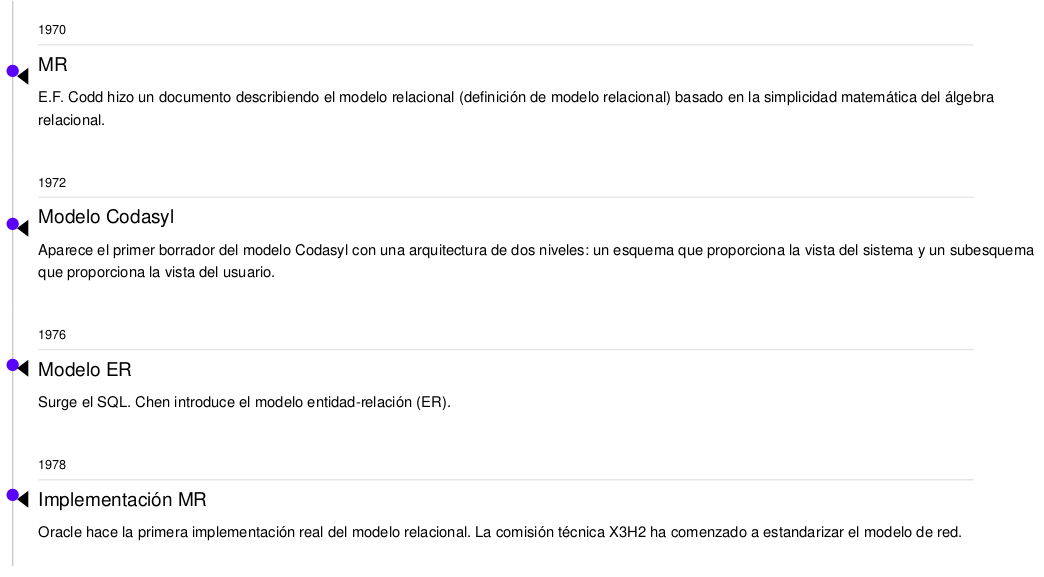
\includegraphics[width=\textwidth]{imagenes/parte2.png}
                  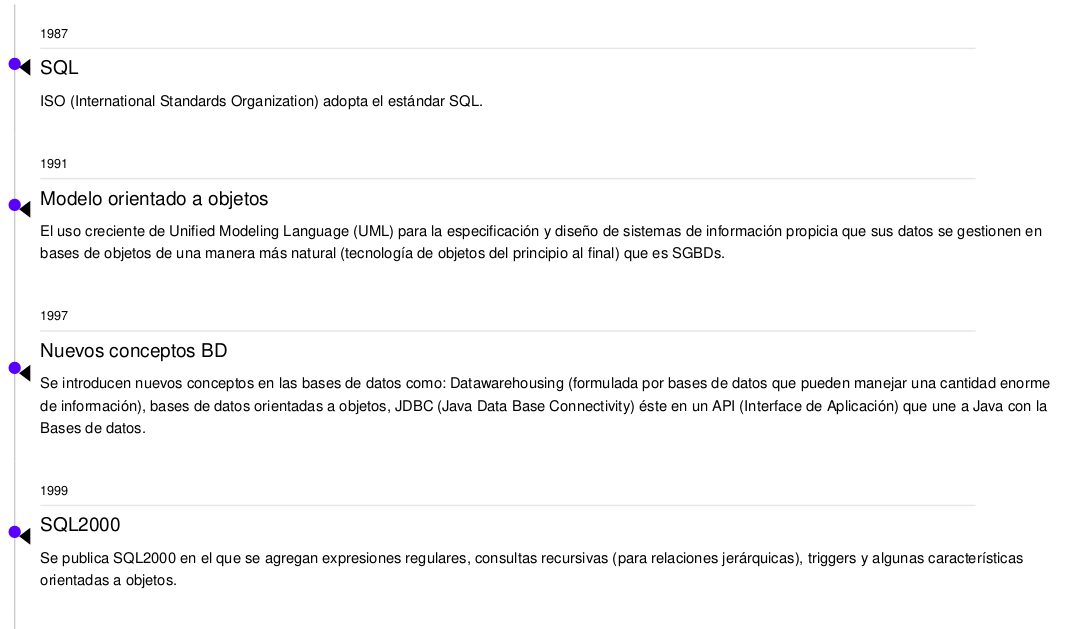
\includegraphics[width=\textwidth]{imagenes/parte3.png}
                  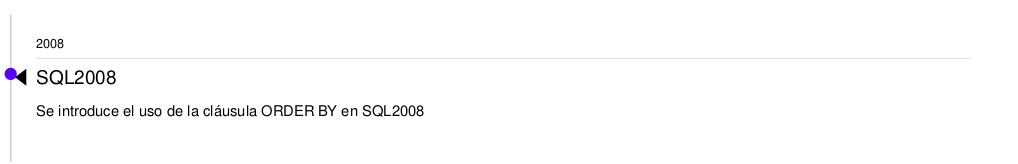
\includegraphics[width=\textwidth]{imagenes/parte4.png}


            \item Indica las responsabilidades que tiene un \textbf{Sistema Manejador de Bases de Datos} y para cada responsabilidad,
            explica los problemas que surgirían sí dicha responsabilidad no se cumpliera.
            \item Supón que un banco pequeño desea almacenarlos su información en una base de datos y le gustaría comprar el
            SMBD que tenga la menor cantidad de características posibles. Está interesado en ejecutar la aplicación en una
            sola computadora personal y no se planea compartir la información con nadie. Para cada una de las siguientes
            características explica por qué se debería o no incluir en el SMBD que desea comprar (suponiendo que se pueden
            comprar por separado:) \textbf{seguridad, control de concurrencia, recuperación en caso de fallas, lenguaje de consulta,
            mecanismo de vistas, manejo de transacciones.}
          \end{enumerate}

            \section{Investigación.}
            \begin{enumerate}[a)]

            \item ¿Qué es la \textbf{Calidad de Datos} y cómo se relaciona con las bases de datos?
            \item ¿Qué son las bases de datos \textbf{NoSQL}? indica el modelo de datos utilizado y algunos proveedores.
            \item ¿Qué es un \textbf{Almacén de datos}? Indica las diferencias entre éstos y una base de datos.

            \end{enumerate}



        \begin{thebibliography}{}

            \bibitem[Example]{Example}

      \end{thebibliography}



    \end{document}
